\begin{figure}[h!]\centering
\captionsetup{width=\textwidth}
\caption{Change in cropped area in selected crops, 2010--2017}
\label{fig:acreage_bars2017}
\vspace{-2mm}
{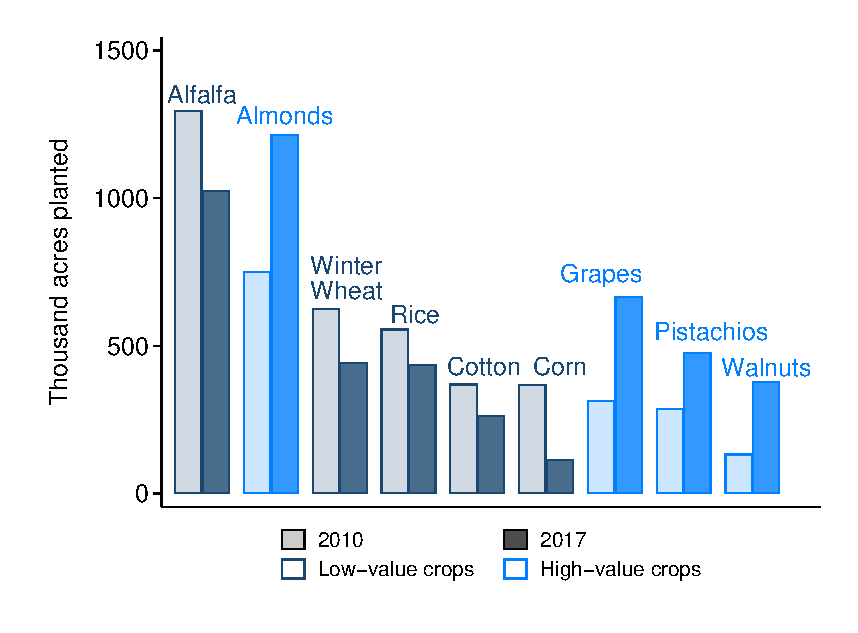
\includegraphics[width=.8\textwidth]{figures/acreage_bars2017_blue.eps}}\\
\captionsetup{width=.85\textwidth}
\caption*{\scriptsize \emph{Notes:} This figure plots the change in cropped area for nine water-intensive California crops from 2010 (light shaded) to 2017 (dark shaded): before and after the historic droughts of the mid-2010s. Crops in dark blue are relatively lower value per acre, while crops in light blue are relatively high value per acre. Acres planted measured using the USDA's Cropland Data Layer.}
\end{figure}